\documentclass[11pt]{article}

\usepackage{a4wide}
\usepackage[utf8]{inputenc}
\usepackage[T2A]{fontenc}
\usepackage[russian]{babel}
\usepackage{graphicx}
\usepackage{color}
\usepackage[left=2.5cm,right=2.5cm,
    top=2.5cm,bottom=2.5cm,bindingoffset=0cm]{geometry}
\usepackage {amsthm}
\usepackage {amsmath}
\usepackage{amssymb}
\usepackage{pb-diagram}

\newtheorem{Def}{Определение}
\newtheorem{statement}{Утверждение}
\newtheorem{theorem}{Теорема}
\newenvironment{Proof}
{\par\noindent{\bf Доказательство.\\}} 
{\begin{flushright}$\Box$\end{flushright}}

\definecolor{gray}{rgb}{0.5,0.5,0.5}

\newcommand\Set[2]{\left\{ #1 \mid #2 \right\}}
\newcommand\Ref[1]{(\ref{#1})}
\newcommand\ftw[2]{\overline{#1,#2}}
\newcommand\RS{\Ref{system} }
\newcommand\beq{\begin{equation}}
\newcommand\eeq{\end{equation}}
\newcommand\dd[2]{\frac{\partial#1}{\partial#2}}

\begin{document}

\thispagestyle{empty}

\begin{center}
\ \vspace{-3cm}

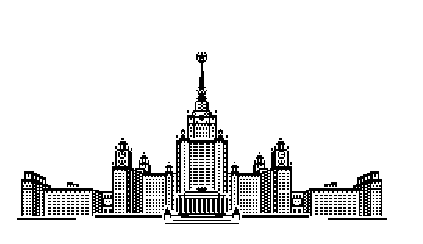
\includegraphics[width=0.5\textwidth]{msu.eps}\\
{\scshape Московский государственный университет имени М.~В.~Ломоносова}\\
Факультет вычислительной математики и кибернетики\\
Кафедра системного анализа

\vfill

{\LARGE Выпускная квалификационная работа по теме}

\vspace{1cm}

{\Huge\bfseries <<Управление в моделях межвидового взаимодействия>>}
\end{center}

\vspace{1cm}

\begin{flushright}
  \large
  \textit{Студентка 415 группы}\\
  Т.~Е.~Морозова
  \textit{Научный руководитель}\\
  к.ф.-м.н., доцент И.~В.~Рублёв 

  \vspace{5mm}

 \end{flushright}

\vfill

\begin{center}
Москва, 2018
\end{center}

\newpage
\tableofcontents
\newpage

%=============Введение============
\section{Введение}

Рассматривается модель пищевой цепи с управлением без внутривидовой конкуренции, состоящая из четырех звеньев и описываемая следующей системой:

\beq
\left\{
\begin{aligned}
\label{system}
	\dot x_1 &= x_1(r_1 + u_1- b_1x_2), \\
	\dot x_2 &= x_2(-r_2 - b_2x_3 + c_2x_1), \\
	\dot x_3 &= x_3(-r_3 + u_2 - b_3x_4 + c_3x_2), \\
	\dot x_4 &= x_4(-r_4 + c_4x_3).
\end{aligned}
\right.
\eeq

Здесь $x_i,\, i = \ftw{1}{4}$ --- численности популяций видов, $r_1 + u_1$ --- рождаемость первого вида,  $r_2, r_3-u_2, r_4$ --- смертности остальных видов, $b_1, b_2, b_3$ и $c_2, c_3, c_4$ отвечают за взаимодействие между популяциями. Все параметры строго положительны, а управления берутся из интервалов $U_1^* = [u_1^{min}, u_1^{max}], U_2^* = [u_2^{min}, u_2^{max}]$ соответственно.

В данной работе основной целью является исследование свойств и синтеза управления для задачи быстродействия во множество положений равновесия.

%=============Общие свойства===========
\section{Общие свойства системы}

Из биологической интерпретации вытекает, что численность популяции не может быть отрицательной. В следующем утверждении будет показано, что система удовлетворяет этому свойству.

\begin{statement}
	Множество $\Set{x \in \mathbb{R}^4}{x_i > 0, i = \ftw{1}{4}}$ инвариантно относительно системы \RS.
\end{statement}
\begin{Proof}
	Из системы \RS видно, что при обнулении координат, обнуляются соответственно и выражения для $\dot x_i,$ так что координаты не могут поменять знак. Интегрируя в обратном времени, получим, что координаты не могут обнулиться.
\end{Proof}

Рассмотрим положения равновесия \RS как функцию управления: 
\begin{gather}
	P(u) = (P_1(u), P_2(u), P_3(u), P_4(u)),\; \text{где} \notag \\
	P_1(u) = \frac{r_2c_4 + b_2r_4}{c_2c_4}, \;\; P_2(u) = \frac{r_1 + u_1}{b_1}, \;\; P_3(u) = \frac{r_4}{c_4},\;\; P_4(u) = \frac{c_3(r_1+u_1) + (u_2 - r_3)b_1}{b_1b_3}.
\end{gather}

Заметим, что от управления существенно зависят только вторая и четвертая координата, поэтому в дальнейшем будем обозначать $P(u) = (P_1, P_2(u), P_3, P_4(u)).$ \\

Множество положений равновесия $E = \Set{P(u)}{u \in U^*}$ представляет из себя параллелограмм в пространстве $(x_2, x_4).$ В нашей работе мы предполагаем его непустоту, для этого введем ограничение на параметры задачи:
$$P_4(u_1^{min}, u_2^{min}) > 0.$$

Наша задача состоит в исследовании возможности перевода системы \RS во множество $E$ при кусочно-непрерывном управлении из $U_1^*, U_2^*.$ 

В работе \cite{MathBio} найден первый интеграл системы \RS:
\beq
	K(x,u) = x_1 - P_1\ln x_1 + \frac{b_1}{c_2}(x_2 - P_2(u)\ln x_2) + \frac{b_1b_2}{c_2c_3}(x_3 - P_3\ln x_3) + \frac{b_1b_2b_3}{c_2c_3c_4}(x_4 - P_4(u)\ln x_4).
\eeq

Докажем, что функция $K(x,u)$ сильно выпукла по $x$ и имеет минимум по $x$ в точке $(P(u),u).$

\begin{statement}
	Функция $K(x,u)$ сильно выпукла на любом выпуклом ограниченном подмножестве $\mathbb{R}_+^4,$ а ее глобальный минимум по $x$ достигается в точке $(P(u),u).$
\end{statement}
\begin{Proof}
	Рассмотрим гессиан функции $K(x,u):$
	$$H = \text{diag} \left(\frac{P_1}{x_1^2}, \; \frac{P_2(u)b_1}{c_2x_2^2}, \; \frac{P_3b_1b_2}{c_2c_3x_3^2}, \; \frac{P_4(u)}{c_2c_3c_4x_4^2}\right).$$
	Очевидно, он больше нуля при всех $x_i > 0,$ следовательно, функция выпукла.\\
	Обозначим 
	$$K_1(x_1) = x_1 - P_1\ln x_1, \; K_2(x_2,u) = \frac{b_1}{c_2}(x_2 - P_2(u)\ln x_2),$$
	$$K_3(x_3) = \frac{b_1b_2}{c_2c_3}(x_3 - P_3\ln x_3), \; K_4(x_4,u) = \frac{b_1b_2b_3}{c_2c_3c_4}(x_4 - P_4(u)\ln x_4,$$ тогда $K(x,u) =  K_1(x_1) + K_2(x_2,u) + K_3(x_3) + K_4(x_4,u).$  Поскольку 
	$$K_1'(x_1) = 1 - \frac{P_1}{x_1}, \; K_2'(x_2,u) = \frac{b_1}{c_2} - \frac{P_2(u)b_1}{c_2x_2},$$
	$$K_3'(x_3) = \frac{b_1b_2}{c_2c_3} - \frac{b_1b_2P_3}{c_2c_3x_3}, \; K_4'(x_4,u) = \frac{b_1b_2b_3}{c_2c_3c_4} - \frac{b_1b_2b_3P_4(u)}{c_2c_3c_4x_4},$$ 
	глобальный минимум $K_i$ достигается при $x_i = P_i,$ следовательно, глобальный минимум $K(x,u)$ достигается в точке $(P(u),u).$ \\
	 Докажем сильную выпуклость. Возьмем $x_i \leqslant \mu, i = \ftw{1}{4}, \text{где } \mu \geqslant \max\Set{P_i}{i = \ftw{1}{4}}.$ Тогда $H \geqslant \delta\cdot I,$ где  
	 $$\delta = \min\left(P_1, \frac{P_2(u)b_1}{c_2}, \frac{P_3b_1b_2}{c_2c_3}, \frac{P_4(u)b_1b_2b_3}{c_2c_3c_4}\right)/\mu^2.$$
	 Таким образом $\langle Hx,x \rangle \geqslant \langle \delta Ix,x \rangle = \delta \|x\|^2,$ что и завершает доказательство.
\end{Proof}

%Особые режимы
\begin{statement}
	В системе (1) в области $\mathbb{R}_+^4$ не могут возникать особые режимы управления.
\end{statement}
\begin{Proof}
    Выпишем функцию Гамильтона-Понтрягина для нашей системы.
        $$H(\psi, x, u) = \psi_1x_1(r_1 + u_1 - b_1x_2) + \psi_2x_2(-r_2 - b_2x_3 + c_2x_1) + \psi_3x_3(-r_3 + u_2 - b_3x_4 + c_3x_2) + \psi_4x_4(-r_4 + c_4x_3),$$
    
    где  $\psi(t) \in C, \; \psi(t) \ne 0 \; \text{и удовлетворяет сопряженной системе системе:}$
    
    $$
    \left\{
    \begin{aligned}
    	\dot \psi_1 &= -(\psi_1(r_1 + u - b_2x_2) + \psi_2x_2c_2), \\
    	\dot \psi_2 &= -(-b_1\psi_1x_1 + \psi_2(-r_2 - b_2x_3 + c_2x_1) + \psi_3x_3c_3), \\
    	\dot \psi_3 &= -(-b_2\psi_2x_2 + \psi_3(-r_3 + u_2 - b_3x_4 + c_3x_2) + \psi_4x_4c_4), \\
    	\dot \psi_4 &= -(b_3\psi_3x_3 + \psi_4(-r_4 + c_4x_3)).
    \end{aligned}
    \right.$$
    
    Из принципа максимума $H(\psi(t), x(t), u^*(t)) = \sup\limits_{u \in U^*} H(\psi,x,u).$
    
    Посчитаем производную $H$ по $u:$
    
    $$H'_u = (\psi_1x_1, \psi_3x_3) \text{ откуда } u_1^* = \begin{cases} u_1^{max}, & \psi_1x_1 \geqslant 0, \\  u_1^{min}, & \psi_1x_1 < 0.\end{cases}, \;\; u_2^* = \begin{cases} u_2^{max}, & \psi_3x_3 \geqslant 0, \\  u_2^{min}, & \psi_3x_3 < 0.\end{cases}$$
    
    Особый режим будет возникать, если хотя бы одна из компонент управления определяется неоднозначно, то есть либо $\psi_1x_1 = 0,$ либо $\psi_3x_3 = 0$ на ненулевом промежутке времени.
    Так как в нашей системе $x_1$ и $x_3$ положительны, учитываются только $\psi_1, \psi_3.$  
    
    Рассмотрим оба варианта.
    \begin{enumerate}
    \item
        	Пусть $\psi_1(t) = 0, t \in [t_1 t_2].$ Рассмотрим последовательно $\dot \psi_i$ и убедимся, что все сопряженные переменные нулевые.
        
        Если $\psi_1(t) = 0$ на промежутке $[t_1, t_2],$ то $\dot \psi_1 = 0$ на этом же временном отрезке. Но тогда из первого сопряженного уравнения $\psi_2 = 0,$ следовательно и $\dot \psi_2 = 0, \;  t \in [t_1, t_2],$ а тогда из второго сопряженного уравнения $\psi_3 = 0, \;  t \in [t_1, t_2].$ Аналогично $\dot \psi_3 = 0, \;  t \in [t_1, t_2]$ и из третьего сопряженного уравнения $\psi_4 = 0, \;  t \in [t_1, t_2],$ что противоречит невырожденности $\psi(t).$
        
    \item
    	Пусть $\psi_3(t) = 0, \psi_1(t) \ne 0, t \in [t_1 t_2],$ тогда и $\dot \psi_3(t) = 0$ на том же временном отрезке. Таким образом $-b_2\psi_2x_2 + \psi_4x_4c_4 = 0.$ Возьмем производную по времени от этого выражения:
    	\begin{multline*}
    		0 = -b_2(\dot \psi_2x_2 + \psi_2 \dot x_2) + c_4(\dot \psi_4 x_4 + \psi_4 \dot x_4) = \\
    		= -b_2(-x_2(-b_1\psi_1x_1 + \psi_2(-r_2 - b_2x_3 + c_2x_1)) + \psi_2 x_2(-r_2 - b_2x_3 + c_2x_1)) + \\
    		+ c_4(\psi_4x_4(-r_4 + c_4x_3) + \psi_4x_4(-r_4 + c_4x_3)) = -b_1b_2x_1x_2\psi_1.
    	\end{multline*}
    	
    	Но $x_1, x_2, \psi_1 \ne 0,$ а значит, мы получили противоречие, что и завершает доказательство.
    
    \end{enumerate}    
\end{Proof}

%Вернемся к нашим баранам
Вернемся к $K(x,u).$ Уменьшая ее, мы будем приближаться к положению равновесия. 
Посчитаем производную $\frac{dK(x,u^0)}{dt}$ при некотором $u^0 = (u_1^0, u_2^0)$ в силу системы \RS:

\begin{multline*}
    \frac{dK(x,u_0)}{dt} = \dd{K(x,u_0)}{x_1}\dot x_1 + \dd{K(x,u_0)}{x_2}\dot x_2 + \dd{K(x,u_0)}{x_3}\dot x_3 + \dd{K(x,u_0)}{x_4}\dot x_4 = \\
    = -\frac{1}{c_2c_3c_4}\left((u_2 - u_2^0)(b_1b_2(r_4 - c_4x_3)) + c_3(u_1 - u_1^0)(b_2r_4 + c_4r_2 - c_2c_4x_1)\right) = \\
    = \frac{b_1b_2}{c_2c_3}(u_2 - u_2^0)(x_3 - P_3) + (u_1 - u_1^0)(x_1 - P_1).
\end{multline*}

Заметим, что равновесие по $x_1$ и $x_3$ разделяет все пространство на четыре области, в каждой из которых будет свой минимизатор.
\begin{enumerate}
\item
	В области $x_1 > P_1, \, x_3 > P_3$ производная будет минимальной при $u_1 = u_1^{min}, \, u_1^0 = u_1^{max}, \, u_2 = u_2^{min}, \, u_2^0 = u_2^{max}.$
\item
	В области $x_1 > P_1, \, x_3 < P_3$ производная будет минимальной при $u_1 = u_1^{min}, \, u_1^0 = u_1^{max}, \, u_2 = u_2^{max}, \, u_2^0 = u_2^{min}.$
\item
	В области $x_1 < P_1, \, x_3 > P_3$ производная будет минимальной при $u_1 = u_1^{max}, \, u_1^0 = u_1^{min}, \, u_2 = u_2^{min}, \, u_2^0 = u_2^{max}.$
\item
	В области $x_1 < P_1, \, x_3 < P_3$ производная будет минимальной при $u_1 = u_1^{max}, \, u_1^0 = u_1^{min}, \, u_2 = u_2^{max}, \, u_2^0 = u_2^{min}.$
\end{enumerate}

Введем 4 функции:
$$K_1(x) = K(x,u_1^{min}, u_2^{min}), \, K_2(x) = K(x,u_1^{max}, u_2^{min}),$$ 
$$K_3(x) = K(x,u_1^{min}, u_2^{max}), \, K_4(x) = K(x,u_1^{max}, u_2^{max}).$$

Беря управление, минимизирующее производную $\frac{dK, u^0}{dt}$ в соответствующей области, мы будем уменьшать три функции, а четвертая будет постоянной. Процесс будет повторяться до тех пор, пока мы не попадем на положение равновесия, где все четыре функции станут постоянными. 

%=========Скользящие режимы========

Однако неопределенность возникает на самих гиперповерхностях $x_1 = P_1, x_3 = P_3.$ Если возникает скользящий режим, то управлять системой становится затруднительно ввиду неоднозначности управления. 

Рассмотрим подробнее, когда возникают скользящие режимы. Перепишем нашу систему в виде:
$$\dot x(t) = \begin{cases} f_1(x), & \sigma(x,t) < 0 \\ f_2(x), & \sigma(x,t) > 0.\end{cases}$$
Достаточное условие скользящего режима на отрезке $x \in [a, b]$ в этом случае будет:
$$
\left\{
\begin{aligned}
    \lim_{\sigma \to 0+0}\dd{\sigma(x,t)}{x} f_2(x) < 0 \\
    \lim_{\sigma \to 0-0} \dd{\sigma(x,t)}{x} f_1(x) > 0.
\end{aligned}
\right.
\;\;\; \forall x \in [a, b] \subset \Set{x}{\sigma(x,t) = 0}
$$

Таким образом мы можем рассматривать динамическую систему следующего вида:
$$\dot x(t) = \begin{cases} f_1(x), & \sigma(x,t) < 0 \\ f_s(x), & \sigma(x,t) = 0 \\ f_2(x), & \sigma(x,t) > 0.\end{cases}$$

Регуляризуем скользящий режим таким образом, чтобы не уходить с линии переключения. Для этого применим метод продолжения Филиппова:

$$f_s(x) = \alpha f_1(x) + (1 - \alpha) f_2(x), \text{  где}$$
$$\alpha \in [0, 1] : \dd{\sigma(x,t)}{x} f_s(x) = 0$$
$$\alpha = \frac{\langle \nabla(\sigma), f_1\rangle}{\langle \nabla(\sigma), f_1 - f_2 \rangle}.$$

Будем рассматривать отдельно случай скользящего режима по первой координате и по третьей.

В первом случае 
$f_1(x) = f(x,u_1^{max}, u_2^0), \; f_2(x) = f(x,u_1^{min}, u_2^0), \sigma(x,t) = \sigma(x) = x_1 - P_1.$

%$$
%\left\{
%\begin{aligned}
%\label{system}
%	f_1^1 &= x_1(r_1 + u_1^{max}- b_1x_2), \\
%	f_1^2 &= x_2(-r_2 - b_2x_3 + c_2x_1), \\
%	f_1^3 &= x_3(-r_3 + u_2^0 - b_3x_4 + c_3x_2), \\
%	f_1^4 &= x_4(-r_4 + c_4x_3).
%\end{aligned}
%\right. \;\;
%\left\{
%\begin{aligned}
%\label{system}
%	f_2^1 &= x_1(r_1 + u_1^{min}- b_1x_2), \\
%	f_2^2 &= x_2(-r_2 - b_2x_3 + c_2x_1), \\
%	f_2^3 &= x_3(-r_3 + u_2^0 - b_3x_4 + c_3x_2), \\
%	f_2^4 &= x_4(-r_4 + c_4x_3).
%\end{aligned}
%\right. \;\;\;\;
%\sigma(x,t) = \sigma(x) = x_1 - P_1.
%$$
Мы предполагаем, что по $x_3$ скользящего режима \textcolor{gray}{пока} нет и вторая компонента управления определяется однозначно.

Тогда получим, что скользящий режим возникает при 
$$
\left\{
\begin{aligned}
	\lim_{x_1 - P_1 \to 0 + 0} x_1(r_1 + u_1^{min} - b_1x_2) > 0, \\
	\lim_{x_1 - P_1 \to 0 - 0} x_1(r_1 + u_1^{max} - b_1x_2) < 0, \\
\end{aligned}
\right.
$$
откуда $P_2(u_1^{min}) < x_2 < P_2(u_1^{max}).$

То есть при таких $x_2$, если мы находимся вблизи гиперповерхности $x_1 = P_1$ с соответствующей стороны, у нас возникает по первой координате скользящий режим. Тогда, применяя метод Филиппова, получим 
$$
\dot x(t) = \begin{cases} f_1(x), & \sigma(x,t) < 0 \\ \alpha_1 f_1(x) + (1 - \alpha_1) f_2(x), & \sigma(x,t) = 0 \\ f_2(x), & \sigma(x,t) > 0\end{cases} \; \Leftrightarrow \; \dot x(t) = \begin{cases} f(x,u_1^{max}, u_2^0), & \sigma(x,t) < 0 \\ f(x, \alpha_1 u_1^{min} + (1-\alpha_1)u_1^{max}, u_2^0), & \sigma(x,t) = 0 \\ f(x, u_1^{min}, u_2^0), & \sigma(x,t) > 0.\end{cases}
$$

$$\alpha_1 = \frac{r_1 + u_1^{max} - b_1x_2}{u_1^{max} - u_1^{min}}.$$

Во втором случае аналогично получим, что скользящий режим по третьей координате возникает, если $$d_{min}(x_2) = \frac{c_3x_2 - r_3 + u_2^{min}}{b_3} < x_4 < \frac{c_3x_2 - r_3 + u_2^{max}}{b_3} = d_{max}(x_2).$$

После регуляризации получаем
$$
\dot x(t) = \begin{cases} f(x,u_1^0, u_2^{max}), & \sigma(x,t) < 0 \\ f(x, u_1^0, \alpha_2 u_2^{min} + (1-\alpha_2)u_2^{max}), & \sigma(x,t) = 0 \\ f(x, u_1^0, u_2^{min}), & \sigma(x,t) > 0.\end{cases}
$$

$$\alpha_2 = \frac{-r_3 + u_2^{max} - b_3x_4 + c_3x_2}{u_2^{max} - u_2^{min}}.$$

%sliding behaviour

%=========Конечность процесса=========

Докажем, что за конечное время мы придем в положение равновесия, то есть с какого-то момента времени функции $K_i$ cтанут постоянными. Для этого 
\begin{enumerate}
	\item докажем, что время нахождения в скользящих процессах отдельно по первой и третьей координате конечно,
	\item оценим скорость убывания $K(t,u)$ вне скользящих режимов снизу.
	%возможно, в \epsilon-окрестности, а в ней как-то докажем конечность процесса.
\end{enumerate}

{\bf Замечание.} Мы рассматриваем скользящие режимы либо по первой, либо по третьей координате, так как в случае одновременного скольжения по обеим координатам задача решена. \\
\textcolor{gray}{Тут надо это пояснять или это слишком очевидно?}\\

{\bf Скользящий режим по $x_3$.}

\beq
\label{d_minmax}
	x_3 = P_3, \; x_4 \in [d_{min}(x_2), d_{max}(x_2)].
\eeq

Заметим что $\dot x_4 = 0,$ так что $x_4 = x_4^*$ и наша система превращается в двумерную:

$$
\left\{
\begin{aligned}
	\dot x_1 &= x_1(r_1 + u_1- b_1x_2) &= b_1x_1(P_2(u_1) - x_2), \\
	\dot x_2 &= x_2(-r_2 - b_2x_3 + c_2x_1) &= c_2x_2(x_1 - P_1).
\end{aligned}
\right.
$$

Выражаем $x_2$ через $x_4^*$ из \Ref{d_minmax}:
$$c_{min}(x_4^*) = \frac{b_3x_4^* + r_3 - u_2^{max}}{c_3} < x_2 < \frac{b_3x_4^* + r_3 - u_2^{min}}{c_3} = c_{max}(x_4^*).$$

Таким образом наша система остается двумерной до тех пор, пока $x_2 \in [c_{min}(x_4^*), c_{max}(x_4^*)]$ и у нас возникает две альтернативы:
\begin{enumerate}
	\item либо $x_2$ никогда не нарушает границы неравенства, и система остается двумерной,
	\item либо существует конечный момент времени, когда одно из неравенств на $x_2$ будет нарушено, и система становится вновь четырехмерной.
\end{enumerate}

Рассмотрим первый случай и докажем, что система за конечное время придет в положение равновесия по $x_1, x_2,$ а значит, и в искомое положение равновесия по всем четырем координатам, что и решает исходную задачу. \\

\textcolor{gray}{Тут будет доказательство из статьи.}\\

{\bf Скользящий режим по $x_1$.}

\beq
\left\{
\begin{aligned}
	x_1 &= P_1, \\
	\dot x_2 &= x_2(-r_2 - b_2x_3 + c_2P_1), \\
	\dot x_3 &= x_3(-r_3 + u_2 - b_3x_4 + c_3x_2), \\
	\dot x_4 &= x_4(-r_4 + c_4x_3), 
\end{aligned}
\right. \;\; \Leftrightarrow \;\;
\left\{
\begin{aligned}
	x_1 &= P_1, \\
	\dot x_2 &= b_2x_2(P_3 - x_3), \\
	\dot x_3 &= x_3(-r_3 + u_2 - b_3x_4 + c_3x_2), \\
	\dot x_4 &= c_4x_4(x_3 - P_3). 	
\end{aligned}
\label{system1}
\right.
\eeq

Заметим, что $\text{sgn}(\dot x_4) = -\text{sgn}(\dot x_2) = \text{sgn}(x_3 - P_3).$ \\
Также заметим, что в случае $x_3 > P_3$ $$\dot x_3 \vee 0 \Leftrightarrow x_4 \vee d_{min}(x_2),$$ а в случае $x_3 < P_3$ $$\dot x_3 \vee 0 \Leftrightarrow x_4 \vee d_{max}(x_2).$$

Таким образом будем рассматривать 4 случая в зависимости от знака $x_3 - P_3$ и $\dot x_3:$

% Тут наверное хорошо бы табличку

\begin{description}
	\item[Случай 1:] $x_3 > P_3, \; \dot x_3 > 0,$
	\item[Случай 2:] $x_3 > P_3, \; \dot x_3 < 0,$
	\item[Случай 3:] $x_3 < P_3, \; \dot x_3 > 0,$
	\item[Случай 4:] $x_3 < P_3, \; \dot x_3 < 0.$
\end{description}

Без ограничения общности будем считать, что скользящий режим по первой координате осуществляется с начального момента времени $t_0$.\\

\underline {\bf Случай 1.} 
$$x_3(t_0) > P_3, \; \dot x_3(t_0) > 0.$$
Из первого неравенства следует, что $\dot x_2(t_0) < 0, \dot x_4(t_0) > 0,$ а из второго --- что $x_4(t_0) < d_{min}(x_2).$

Таким образом $\dot x_3(t) > 0, \forall t : x_4(t) < d_{min}(x_2),$ поэтому, пока $x_4 < d_{min}(x_2)$, $ x_3 \geqslant x_3(t_0) - P_3 = a_1 > 0.$ Тогда $\dot x_4 \geqslant c_4x_4(t_0)a_1, \dot x_2 < 0 \Rightarrow d_{min}(x_2) < d_{min}(x_2(t_0)),$ тогда мы можем оценить $t_1 \leqslant \frac{d_{min}(x_2(t_0)) - x_4(t_0)}{c_4x_4(t_0)a_1}$ --- время, за которое $x_4$ дойдет до $d_{min}(x_2)$.\\
Рассмотрим момент $t_1.$ \\
$\dot x_3(t_1) = 0,$ но $\ddot x_3(t_1) = \dot x_3(t_1)((-r_3 + u_2 - b_3x_4(t_1) + c_3x_2(t_1)) + x_3(t_1)(-b_3\dot x_4(t_1) + c_3 \dot x_2(t_1)) < 0,$ так что $\forall \Delta_1 > 0 \; \dot x_3(t_1 + \Delta_1) < 0,$ при этом $x_3(t_1 + \Delta_1) > P_3,$ так что теперь возникает случай 2.\\

\underline{\bf Случай 2.}
$$x_3(t_1) > P_3, \dot x_3(t_1) < 0.$$
Из первого неравенства следует, что $\dot x_2(t_1) < 0, \dot x_4(t_1) > 0,$ а из второго --- что $x_4(t_1) > d_{min}(x_2(t_1)).$ Докажем, что 
\begin{itemize}
	\item либо $\exists t_2 < \infty:  x_3(t_2) = P_3,$
	\item либо $\forall \varepsilon > 0 \: \exists t_2' : x_3(t) - P_3 < \varepsilon \; \forall t > t_2'.$
\end{itemize}
Предположим противное: $\forall t > t_1 \; x_3(t) > P_3 + \delta, \delta > 0.$ Тогда $\dot x_2(t) < b_2x_2\delta < 0,$ поэтому $\exists t_2^* : x_2(t_2^*) < P_2^{min},$ но тогда мы выходим из скользящего режима по первой координате, а значит, возвращаемся к уже рассмотренным вариантам.

Случай, когда $x_3$ попадает в $\varepsilon$-окрестность $P_3$ приводит нас в положение равновесия по всем координатам с точностью до бесконечно малой величины.

Если же $\exists t_2 : x_3(t_2) = P_2,$ то в зависимости от того, где в этот момент находится четвертая координата, мы либо решили задачу, либо переходим к случаю 4:
\begin{itemize}
	\item $x_4(t_2) \in [d_{min}(x_2(t_2)), d_{max}(x_2(t_2))], \; x_3(t_2) = P_3, \; x_2(t_2) \in [P_2^{min}, P_2^{max}], \; x_1(t_2) = P_1 \Rightarrow x(t_2) = P(u).$
	\item $x_4(t_2) > d_{max}(x_2(t_2)) \Rightarrow \dot x_3(t_2) < 0, \; \forall \Delta_2 > 0 \; x_3(t_2 + \Delta_2) < P_3 \Rightarrow$ переходим к случаю 4, заменив $t_2 + \Delta_2$ на $t_2$.
\end{itemize}

\underline{\bf Случай 4.}
$$x_3(t_2) < P_3, \dot x_3(t_2) < 0.$$
Из первого неравенства следует, что $\dot x_2(t_2) > 0, \dot x_4(t_2) < 0,$ а из второго --- что $x_4(t_2) > d_{max}(x_2(t_2)).$

Аналогично случаю 1 $\dot x_3(t) < 0, \forall t : x_4(t) > d_{max}(x_2),$ поэтому, пока $x_4 > d_{max}(x_2)$, $ x_3 \leqslant x_3(t_2) - P_3 = a_2 < 0.$ Тогда $\dot x_4 \leqslant -c_4x_4(t_2)a_2, \dot x_2 > 0 \Rightarrow d_{max}(x_2) > d_{max}(x_2(t_2)),$ тогда $\exists t_3 : x_4(t_3) = d_{max}(x_2).$ \\
Рассмотрим момент $t_3.$ \\
$\dot x_3(t_3) = 0,$ но $\ddot x_3(t_3) = \dot x_3(t_3)((-r_3 + u_2 - b_3x_4(t_3) + c_3x_2(t_3)) + x_3(t_3)(-b_3\dot x_4(t_3) + c_3 \dot x_2(t_3)) > 0,$ так что $\forall \Delta_3 > 0 \; \dot x_3(t_3 + \Delta_3) > 0,$ при этом $x_3(t_3 + \Delta_3) < P_3,$ так что теперь возникает случай 3.\\

\underline{\bf Случай 3.}
$$x_3(t_3) < P_3, \dot x_3(t_3) > 0.$$
Из первого неравенства следует, что $\dot x_2(t_3) > 0, \dot x_4(t_3) < 0,$ а из второго --- что $x_4(t_3) < d_{max}(x_2(t_3)).$

Как и в случае 2, мы можем доказать, что 
\begin{itemize}
	\item либо $\exists t_4 < \infty:  x_3(t_4) = P_3,$
	\item либо $\forall \varepsilon > 0 \: \exists t_4' : x_3(t) - P_3 < \varepsilon, \forall t > t_4'.$
\end{itemize}

Однако в данном случае реализуется только первый пункт, то есть всегда существует конечный момент времени, в который $x_3 = P_3.$ Докажем невозможность второго пункта. Рассмотрим $\ddot x_3(t), \; t > t_3.$
$$\ddot x_3(t) = \dot x_3(t)((-r_3 + u_2 - b_3x_4(t) + c_3x_2(t)) + x_3(t)(-b_3\dot x_4(t) + c_3 \dot x_2(t)) > 0 \; \forall t : x_3(t) < P_3, $$ 
так как $\dot x_3(t)((-r_3 + u_2 - b_3x_4(t) + c_3x_2(t)) \geqslant 0 \; \forall t, \; x_3(t) > 0 \; \forall t, \; \dot x_4(t) < 0, \dot x_2(t) > 0 \; \forall t : x_3(t) < P_3.$
Таким образом невозможно асимптотическое приближение к положению равновесия, как в случае 2. Но как и в случае 2, дальнейшая динамика системы зависит от $x_4(t_4):$

\begin{itemize}
	\item Если $x_4(t_4) \in [d_{min}(x_2(t_4)), d_{max}(x_2(t_4))], \; x_3(t_4) = P_3, \; x_2(t_4) \in [P_2^{min}, P_2^{max}], \; x_1(t_4) = P_1 \Rightarrow x(t_4) = P(u).$
	\item Если $x_4(t_4) < d_{min}(x_2(t_4)) \Rightarrow \dot x_3(t_4) > 0, \; \forall \Delta_4 > 0 \; x_3(t_4 + \Delta_4) > P_3 \Rightarrow$ переходим к случаю 1, заменив $t_4 + \Delta_4$ на $t_0$.
\end{itemize}

Таким образом схематично мы можем изобразить, как один случай сводится к другому, на следующей диаграмме, где состояние F означает решение задачи, а $\varepsilon$ --- попадание в $\varepsilon$-окрестность положения равновесия:

\[
\begin{diagram}
\node{1} \arrow[4]{e}{}
\node[4]{2} \arrow[3]{s}{} \arrow[1]{wsw} \arrow[2]{sw}\\
\node[3]{\varepsilon}\\
\node[3]{F}\\
\node{4} \arrow[3]{n}{} \arrow[1]{ene} 
\node[4]{3} \arrow[4]{w}
\end{diagram}
\]

Остается доказать, что невозможен вариант, при котором мы никогда не придем ни в одно из конечных состояний, то есть зациклимся.

\textcolor{gray}{Вот тут возникает проблема, я не знаю, как это доказать аккуратно. По идее, тут можно как-то из соображений уменьшения K это сделать, но надо подумать.} \\

{\bf Скорость вне скользящих режимов.} \\

Отсутствие скользящих режимов эквивалентно следующей системе:

$$
	\left\{
	\begin{aligned}
		&\left[
		\begin{aligned}
			& \;\;\;\; x_1 \ne P_1, \\
			&\left\{
			\begin{aligned}
				x_1 &= P_1, \\
				x_2 & \in [P_2^{min}, P_2^{max}], 
			\end{aligned}
			\right.
		\end{aligned}
		\right. \\
		&\left[
		\begin{aligned}
			& \;\;\;\; x_3 \ne P_3, \\
			&\left\{
			\begin{aligned}
				x_3 &= P_3, \\
				x_4 & \in [d_{min}(x_2), d_{max}(x_2)].
			\end{aligned}
			\right.
		\end{aligned}
		\right.
	\end{aligned}
	\right.
$$

Если $|x_1 - P_1| > \delta_1$ или $|x_3 - P_3| > \delta_3,$ то 

$$
	\frac{dK(x,u)}{dt} \leqslant \begin{cases} -a_1 = -\delta_1(u_1^{max} - u_1^{min}), &  |x_1 - P_1| > \delta_1 \\ -a_2 = -\delta_3\frac{b_1b_2}{c_2c_3}(u_2^{max} - u_2^{min}), & |x_3 - P_3| > \delta_3, \end{cases}
$$
т.е.
$$\frac{dK(x,u)}{dt} \leqslant \min(-a_1, -a_2).$$

\textcolor{gray}{Осталось рассмотреть случаи, когда $$x_1 \approx P_1, x_3 \approx P_3$$ и $$x_1 = P_1, x_3 = P_3, \text{ но } x_2 \notin [P_2^{min}, P_2^{max}], x_4 \notin [d_{min}(x_2), d_{max}(x_2)].$$
В принципе, это можно сделать аналитически, но опять же надо аккуратно расписывать все. Но если смотреть на картинки, то понятно, что там происходит, так что, наверное, это можно как-то адекватно описать.}

%===========Библиография============
\clearpage
\newpage
\begin{thebibliography}{0}
\bibitem{MathBio} {\it Massarelli~N., Hoffman~K., Previte~J.~P.} Effect of parity on productivity and sustainability of Lotka–Volterra food chains. // Mathematical Biology. December of 2014. 1609--1626.
\end{thebibliography}










\end{document}